\subsection{Technical Overview of Microsoft Azure}
%
Microsoft leveraged its constantly-growing worldwide network of data centers to create Azure, a cloud platform that facilitates building, deploying, and managing services and applications anywhere. At its core, Azure is a public cloud computing platform—with solutions including Infrastructure as a Service (IaaS), Platform as a Service (PaaS), and Software as a Service (SaaS) and we can use these for services such as analytics, virtual computing, storage, networking, and much more. These services are used to supplement an on-premise server or replace it.

A CI-CD architecture is implemented in Microsoft Azure as a culmination of two azure services. Those are Azure Portal and Azure DevOps. The steps or tasks of a CI-CD pipeline are configured in the Azure DevOps service, and the application is deployed in a resource inside Azure Portal. However, there are also options to deploy the application in other places such as AWS, GCP, or even on-premise servers. 
%

\subsubsection{Azure Portal [Shoaib Bin Anwar]}
%
There are many ways to control azure, but the easiest way is the Azure Portal. Because the Azure portal is a web-based graphical user interface, so we need to go to the Azure portal website to access and control instead of CLI tools. With the help of the Azure portal, it's possible to manage all the resources in an Azure subscription. It also provides custom dashboards for an organized view of resources and tools like the azure monitor to inspect the performance of an application.

The main strength of the Azure portal is continuous availability. It has an instance available in every Azure data center, making the Azure portal immune to individual failures.\footnote{\url{https://docs.microsoft.com/en-us/azure/azure-portal/azure-portal-overview}}
%

\subsubsection{Azure DevOps [Shoaib Bin Anwar]}
%
The Azure DevOps platform is a platform created by Microsoft as a software-as-a-service(SaaS) that provides a tool-set with an end to end DevOps environment for developing, integrating and deploying software on a continuous integration and a continuous deployment pipelines. It promotes a culture and set of practices  that bring all stakeholder together to complete software development and release process. 

Moreover it integrates with almost any industry leading DevOps tools available in the marketplace, such as Docker Registry, Kubernetes, Auzre portal, Terraform, Ansible, GitHub etc.\footnote{\url{https://www.devopsgroup.com/insights/resources/tutorials/all/what-is-azure-devops/}}
%

\subsubsection{Azure DevOps Key Services [Shoaib Bin Anwar]}
%
The Azure DevOps platform consists of a few key services such as: Azure Boards, Azure Repos, Azure Pipelines, Azure Test Plans, Azure Artifacts.\footnote{\url{https://www.simplilearn.com/azure-devops-article}}

%

\subsubsection{Azure Boards [Shoaib Bin Anwar]}
%
Azure Boards is a service of Azure DevOps through which it is possible to manage software by plan, track, and release. Teams can stay focus on delivering projects with customizing scrum boards. There are some features like backlog, sprints, etc. for the solution of software. \footnote{\url{https://www.c-sharpcorner.com/article/azure-devops-boards/}}
%
\subsubsection{Azure Repos [Shoaib Bin Anwar]}
%
Azure DevOps Repos are a set of repositories that provides the functionality of version control and managing a projects code. It helps to work and coordinate code changes across team. It will allow users to to monitor code, solutions, builds, commits, pushes, Pull requests and branching information about projects. 

Azure Repos provides two types of version control and they are Git and Team Foundation Version Control.

% 

\subsubsection{Azure Pipelines [Shoaib Bin Anwar]}
%
Azure Pipelines is a service that caters the need for creating pipelines on Azure Cloud Platform so that it's possible to build, test and deploy code project automatically. There are three key distinct advantages of using Azure DevOps pipelines:\footnote{\url{https://docs.microsoft.com/en-us/azure/devops/pipelines/get-started/what-is-azure-pipelines?view=azure-devops}}

 \begin{enumerate}
     \item Version Control System : Azure Pipelines integrates with GitHub, GitHub Enterprise, Azure Repos Git, TFVC, Bitbucket Cloud and Subversion.
     \item Language and application types : Azure Pipeline is compatible with most application types and languages, such as Java, JavaScript, Node.js, Python, .Net, C++, Go, PHP, etc.
     \item Deployment Target :  Azure Pipelines can be used to deploy project code to multiple targets. such as, container registries, virtual machines, Azure services, or any on-premises or cloud target.
 \end{enumerate}
 
 Azure Pipeline is based on a few concepts, represented by a few keywords such as Pipeline, Stage, Job, Step, Agent, Artifact. Trigger, Runs, etc. After commits and push to the git repository, a build starts in the Azure pipeline in the Azure DevOps dashboard.
 

\subsubsection{Azure Test Plans [Md Saiful Ambia Chowdhury]}
%
Azure Test Plan is a browser-based test management solution for exploratory, planned manual, and user acceptance testing. It provides a browser extension for exploratory testing and gathering feedback from stakeholders. Test Plans are an incredible place for a development team to do their manual testing.\footnote{\url{https://docs.microsoft.com/en-us/azure/devops/test/create-a-test-plan?view=azure-devops}}

For automated testing as part of the CI/CD workflow, Azure Pipelines is the best option. However, Manual and exploratory testing are still a significant part of evaluating the quality of a product. Azure Test Plans in Azure DevOps provides three main types of test management artifacts: Test plans, Test suits, and Test cases. 

%

\subsubsection{Azure Artifacts [Md Saiful Ambia Chowdhury]}
%
Azure Artifacts is an extension that facilitates the discovery, installation and publication of NuGet, NPM and Maven packages in Azure DevOps. It’s highly incorporated with other hubs like Build so that package management can become a smooth part of existing workflows.\footnote{\url{https://azure.microsoft.com/en-us/services/devops/artifacts/}}
%

\subsubsection{DevOps Workflow Diagram [Md Saiful Ambia Chowdhury]}
%
\begin{figure}[h]
    \centering
    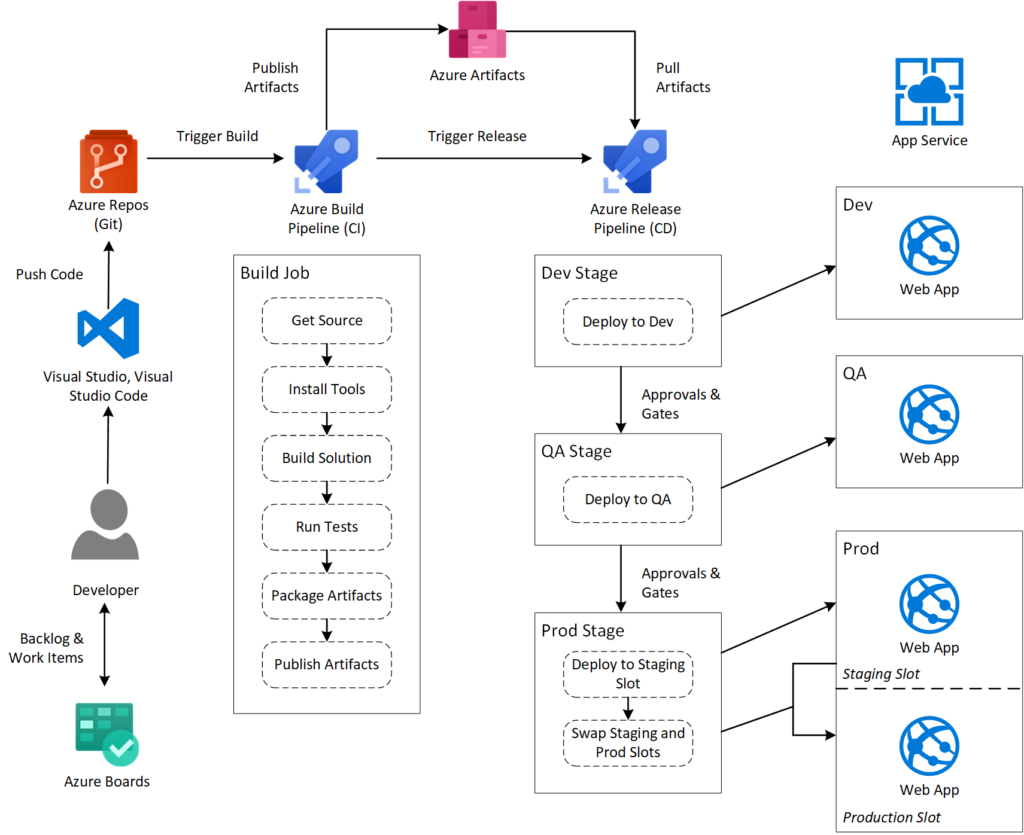
\includegraphics[width=13cm]{images/saiful/azure-devops-ci-cd-pipeline-workflow.png}
    \caption{Azure DevOps CI-CD workflow}
    \label{fig:azure-devops-ci-cd-pipeline-workflow}
\end{figure}

In Azure DevOps, developers manage and keep track of their tasks and backlogs by using the azure boards service. The source code is developed in a local environment. Azure provides seamless integration with most of the popular IDEs like VS Code, Intellij Idea, and Eclipse through extension. Whenever a new commit is pushed to the Azure Repos service, it triggers a new build job at Azure Pipelines. A build job can have many stages like installing tools, testing, and more. These steps in a build job can be defined manually by a developer in an azure CI pipeline. After the build is complete, the generated application artifacts are stored in the azure artifacts service. Continuous Delivery pipeline is also configured in the azure pipeline service. Whenever a CD pipeline is triggered, it fetches all the necessary artifacts from the azure artifacts service, and it deploys the application in a pre-configured environment. These environments are used to define and isolate development, QA, and production stages in a CI-CD pipeline. These environments are actually stored as a resource group in the Azure portal. \footnote{\url{https://www.veritis.com/wp-content/uploads/2019/02/azure-devops-ci-cd-pipeline-flow-veritis-1024x835.png}}

\begin{figure}[h]
    \centering
    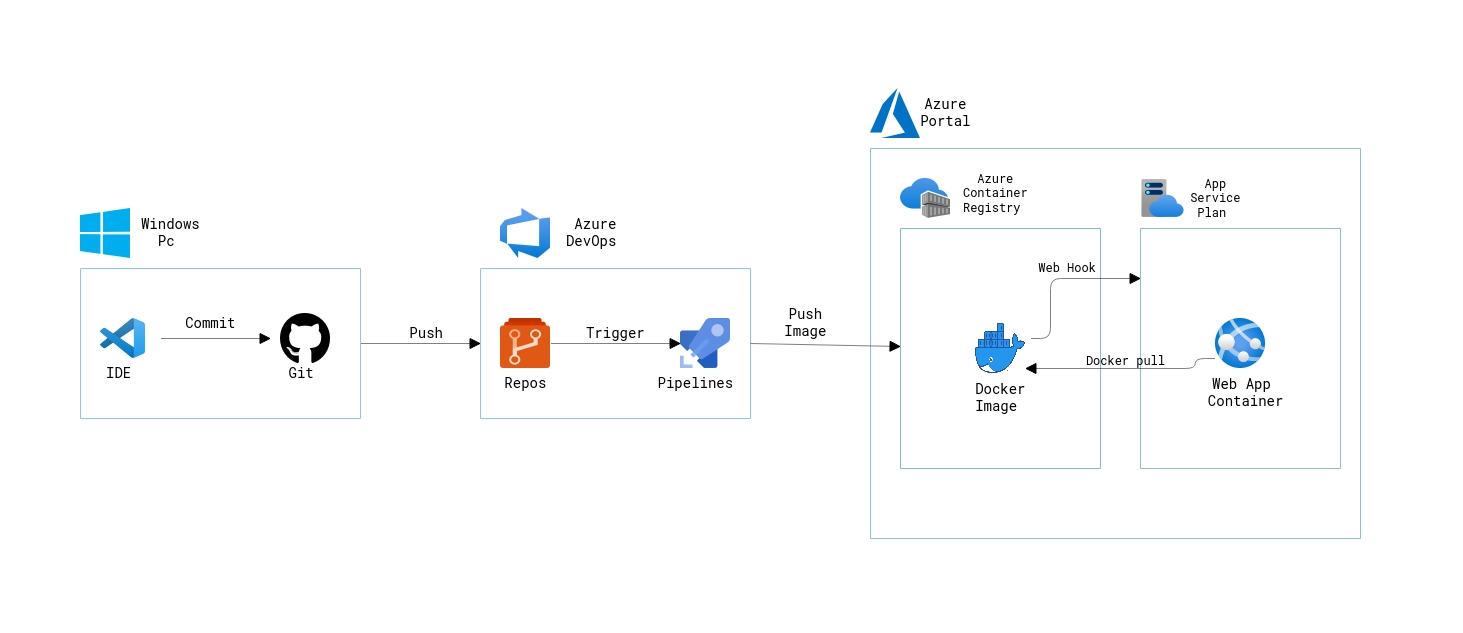
\includegraphics[width=14cm]{images/saiful/Azure_pipeline_diagram_CD.png}
    \caption{Azure DevOps CD to Portal}
    \label{fig:azure-devops-ci-cd-portal}
\end{figure}

After CD pipelines are executed, the application is continuously deployed in the Azure portal. Figure-\ref{fig:azure-devops-ci-cd-pipeline-workflow} represents a CD-CD pipeline that generates a containerized Docker image of the application. This image can be configured to be automatically stored in a public registry like DockerHub, or Azure's own private registry Azure container registry. From where other deployment platforms like Azure App service pan, Azure Kubernetes Service (AKS), Azure container instance (ACI) pulls the image through webhooks and deploys the application. All of these steps can be defined by using the azure pipeline's service, which will automate the entire system.

%

\subsubsection{Advantages [Md Saiful Ambia Chowdhury]}
%
Since Azure DevOps is a Software-as-a-service(SaaS) product, it has many advantages like :\footnote{\url{https://www.softacom.com/en_azure_devops}}
1. No manual infrastructure maintenance is needed. 2. It is much more intuitively clear and user-friendly in comparison to similar platforms. 3. Users don’t need to worry about upgrading or patching up the tool-chain. Thus massive organizations using the DevOps service will not experience any slowdown in CI-CD pipelines.
  
 In Azure DevOps, tasks are categorized based on the nature of the operation. For Instance, Build tasks, Utility tasks, Deploy tasks, etc. This facilitates the user in adding desired tasks to their pipeline in an organized manner.\footnote{\url{https://ymedialabs.medium.com/the-pros-and-cons-of-jenkins-vs-azure-devops-469c66140b4d}}
 It also provides the option to encapsulate a sequence of tasks, already defined in a pipeline, into a single reusable task, just like any other task.
   The Azure DevOps is platform agnostic. Which means, it is designed to run on any platform (Linux, macOS, and Windows) or language (e.g., Android, C/C++, Node.js, Python, Java, PHP, Ruby, .Net, and iOS apps).
Similarly, it is cloud agnostic. That means, Azure DevOps can work in conjunction with AWS and GCP or even with an on-premise server. 
%

\subsubsection{Disadvantages [Md Saiful Ambia Chowdhury]}
%
Azure Pipeline workflow is straightforward. It can’t if-else or switch-case constructions. This makes it more difficult to develop complex workflows. If the project requires exploratory testing such as alpha, beta testing, then the cost structure becomes expensive. Moreover, Documentations of azure are not always up-to-date and sometimes missing. Integration with non-Microsoft tools sometimes can be problematic. 

%

\subsubsection{Price Plans [Md Saiful Ambia Chowdhury]}
%
   Azure DevOps offers two different plans for purchase : 1. Basic Plan, and 2. Basic + Test Plans. The Basic Plan is free for up-to 5 users, from 6 users on-wards the organization will be charged 6 USD per user every month. Basic + Test Plans costs 52 USD per user per month. 
%